\chapter{Marco Te\'orico}\label{chapter:theory}

\section{fMRI}

La resonancia magnética funcional (fMRI) es una técnica no invasiva para estudiar la activación cerebral.Durante el transcurso de la sesión de exploración, se pide al sujeto que realice una determinada tarea, que experimente un estado psicológico o conductual inducido o que simplemente descanse. Mide los cambios en la oxigenación de la sangre y el flujo sanguíneo relacionados con la actividad neuronal, proporcionando medios para estudiar la función del cerebro humano in vivo, ya sea en respuesta a una determinada tarea o en reposo. Durante las últimas dos décadas, la resonancia magnética funcional ha brindado a los investigadores un acceso sin precedentes al funcionamiento interno del cerebro humano, lo que a su vez ha llevado a nuevos conocimientos sobre cómo el cerebro procesa la información.

Los datos adquiridos en un estudio de resonancia magnética funcional consisten en una secuencia de imágenes de resonancia magnética (IRM) tridimensionales, cada una compuesta por una serie de elementos de volumen o vóxeles uniformemente espaciados. Los vóxeles dividen el cerebro en una gran cantidad de cubos del mismo tamaño. Una imagen típica puede constar de aproximadamente 100.000 vóxeles, donde el valor de intensidad de la imagen correspondiente a cada vóxel representa la distribución espacial de la densidad del espín nuclear, que se relaciona con la oxigenación y el flujo de la sangre, en el área local. Durante un experimento de resonancia magnética funcional se obtienen entre 100 y 1.000 imágenes tridimensionales de todo el cerebro. Además, un experimento de resonancia magnética funcional estándar consta de múltiples sujetos (p. ej., 10 - 50), potencialmente llevados a múltiples sesiones de exploración, cada una de las cuales consta de varias replicaciones de una determinada tarea experimental.

Claramente, la cantidad de datos disponibles de un solo experimento es extremadamente grande, y el análisis de los datos de la resonancia magnética funcional es un ejemplo del tipo de problema moderno de big data que está cambiando fundamentalmente las ciencias cuantitativas. Además, los datos exhiben una complicada estructura de ruido temporal y espacial con una señal relativamente débil (aunque, con métodos apropiados, estas señales en todo el cerebro pueden ser altamente predictivas de estados psicológicos y clínicos). Por lo tanto, los datos disponibles no sólo son masivos en escala sino también complejos, lo que hace que el análisis estadístico de los datos de la resonancia magnética funcional sea una tarea difícil.


La capacidad de conectar medidas de activación cerebral, obtenidas mediante fMRI, con la actividad neuronal subyacente que las causó, tendrá un gran impacto en la elección del procedimiento estadístico, así como en las conclusiones posteriores que se puedan extraer del experimento. Por lo tanto, desde una perspectiva de modelado, es fundamental obtener una comprensión básica de la anatom\'ia y  fisiología del cerebro para comprender mejor los datos disponibles. 

El método más popular para realizar fMRI utiliza el contraste dependiente del nivel de oxigenación sanguínea (BOLD) ([50, 28]), medido utilizando la diferencia de señal entre una serie de imágenes ponderadas en T * 2. \todo{explicar esto}

Las im\'agenes BOLD aprovechan las diferencias en las propiedades magn\'eticas de la hemoglobina oxigenada y desoxigenada. A medida que aumenta la actividad neuronal, tambi\'en aumentan las demandas metab\'olicas de ox\'igeno y nutrientes en las regiones afectadas del cerebro. La activaci\'on neuronal indica la extracci\'n de ox\'geno de la hemoglobina en la sangre. Esta extracci\'n hace que la hemoglobina se vuelva paramagn\'etica a medida que los \'atomos de hierro est\'n m\'s expuestos al agua circundante. Esto crea pequeñas distorsiones en el campo magn\'etico que causan una disminuci\'on en T * 2 , lo que lleva a una ca\'ida m\'as r\'pida de la señal y una disminuci\'on local de la señal BOLD. Una sobrecompensaci\'on posterior en el flujo sangu\'ineo aumenta la cantidad de hemoglobina oxigenada, lo que lleva a una reducci\'on de la p\'erdida de señal y un aumento de la señal BOLD en la regi\'on afectada.

BOLD fMRI nos permite estudiar las respuestas hemodin\'amicas a la activaci\'on neuronal. El cambio en la señal de resonancia magn\'etica causado por un evento neuronal generalmente se denomina funci\'on de respuesta hemodin\'amica (HRF). El aumento de las demandas metab\'olicas debido a la actividad neuronal conduce a un aumento en el flujo de sangre oxigenada a las regiones activas del cerebro. Dado que se suministra más ox\'igeno del que realmente se consume, esto conduce a una disminuci\'pn de la concentración de hemoglobina desoxigenada, lo que conduce a un aumento de la señal. Este aumento positivo en la señal comienza aproximadamente 1 a 2 segundos despu\'es del inicio de la actividad neuronal y alcanza su punto m\'aximo 5 a 8 segundos despu\'es del pico de actividad neuronal. Después de alcanzar su nivel m\'aximo, la señal BOLD disminuye a un nivel inferior al inicial que se mantiene durante aproximadamente 10 segundos. Este efecto, conocido como insuficiencia post-est\'imulo, se debe al hecho de que el flujo sangu\'ineo disminuye m\'as r\'apidamente que el volumen sangu\'ineo, lo que permite una mayor concentraci\'on de hemoglobina desoxigenada en regiones del cerebro previamente activas.\todo{demasiado, poner distribuici\'on y f\'omula}

Claramente, la señal BOLD solo proporciona una medida indirecta de la cantidad que realmente buscamos medir, que es la activaci\'on neuronal subyacente. Por lo tanto, es importante comprender qu\'e tan bien la señal BOLD refleja los aumentos reales en la activación neuronal. La respuesta a esta pregunta es compleja, y comprender las bases fisiológicas de la respuesta BOLD ha sido durante mucho tiempo un tema de intenso interés en la investigación. En resumen, se ha demostrado que la señal BOLD se corresponde estrechamente con el potencial del campo eléctrico local que rodea a un grupo de células, lo que probablemente refleje cambios en la actividad postsináptica en muchas condiciones. Sin embargo, en otras condiciones, la actividad neuronal y la señal BOLD pueden desacoplarse. Por lo tanto, es probable que la señal BOLD solo refleje una parte de los cambios en la actividad neuronal en respuesta a una tarea o estado psicológico. Por esta razón, muchas regiones pueden presentar cambios en la actividad neuronal que se pasan por alto porque no cambian la demanda metabólica neta de la región.

Hay varios objetivos comunes en el análisis de datos de fMRI. Estos incluyen localizar regiones del cerebro activadas por una determinada tarea, determinar redes distribuidas que corresponden a la función cerebral y hacer predicciones sobre estados psicológicos o patológicos. Muchos de estos objetivos están relacionados con la comprensión de cómo los estados psicológicos inducidos o medidos conducen a cambios en la actividad cerebral (una combinación de función neuronal y glial), y otros están relacionados con el análisis de fluctuaciones espontáneas en curso. Todos estos objetivos son de naturaleza intrínsecamente estadística, y esta área es el dominio principal de los estadísticos actualmente involucrados en este campo.
%-----------------------------------


fMRI (Resonancia Magnética Funcional): La fMRI es una técnica de neuroimagen que mide la actividad cerebral midiendo los cambios en el flujo sanguíneo relacionados con la actividad neuronal. Los datos fMRI se procesan para obtener la respuesta hemodinámica en forma de betas, que representan la fuerza y dirección de la relación entre la actividad neuronal y la señal de la imagen.

BOLD y HRF \todo{poner}

Modelo Lineal Generalizado (GLM): Es un enfoque estadístico utilizado para modelar la relación entre los estímulos y las respuestas fMRI. Ayuda a identificar áreas del cerebro que están activas en respuesta a ciertos estímulos o tareas.

GMLDenoise: Es una herramienta que se utiliza para mejorar la calidad de los datos fMRI mediante la eliminación de artefactos y ruido, permitiendo una interpretación más precisa de la actividad neuronal.

\section{Mapa Retinot\'opico}
\todo{explicar excentricidad, angulo polar, sigma, areas}
Un mapa retinotópico es una representación bidimensional de la superficie de la retina en una región específica del sistema visual del cerebro. La información visual se organiza de manera topográfica, lo que significa que la posición relativa de las células en la retina se mantiene en la corteza visual. Las ubicaciones cercanas en la retina se proyectan a áreas cercanas en la corteza.

La corteza visual humana está organizada en múltiples mapas retinotópicos. Caracterizar la disposición de estos mapas en la superficie cortical es esencial para muchos estudios de neurociencia visual.

la mayoría de los análisis retinotópicos de datos de resonancia magnética funcional utilizan un enfoque de vóxeles. El método general es (1) medir las respuestas al mapeo de estímulos, (2) derivar coordenadas retinotópicas para cada vóxel o vértice de superficie analizando ondas viajeras (Sereno et al., 1995; Engel et al., 1997b) o resolviendo un modelo de campo receptivo de población (pRF) (Dumoulin y Wandell, 2008) para cada vóxel, y (3) para identificar límites de área mediante inspección visual. Además de requerir mucho tiempo y esfuerzo, los mapas que resultan de este proceso conservan muchas fuentes comunes de error. Debido a las diversas fuentes de ruido, los mapas medidos tienen discontinuidades y a menudo omiten sistemáticamente porciones del campo visual. Estas muchas deficiencias del proceso de mapeo retinotópico tradicional se derivan del hecho de que se organiza en torno a la optimización del poder explicativo de las soluciones de retinotopía a partir de vóxeles individuales, en lugar de todo el campo visual o el área cortical. Como consecuencia, produce mapas que no son uniformes ni completos, ni se basan en ningún contexto de cómo el campo visual se deforma en la superficie cortical. Sin estos datos, la comparación de mapas entre sujetos es difícil y el examen cuantitativo preciso de las diferencias individuales es imposible.

Las respuestas visuales en una parte sustancial del cerebro humano están organizadas en mapas retinotópicos, en los que las posiciones cercanas en el cerebro representan ubicaciones adyacentes en la imagen. La medición precisa de estos mapas mediante imágenes por resonancia magnética funcional (fMRI) es esencial para una amplia gama de aplicaciones clínicas y de neurociencia (Wandell y Winawer, 2011), en las que a menudo proporcionan una base para comparar mediciones entre individuos, grupos, tareas y estímulos. y laboratorios. 

El m\'etodo bayesiano surge por la necesidad de ajustar un mapa retinotópico a la superficie cortical de un sujeto basándose en mediciones, sin intervención humana. 

 Nos referimos a los mapas retinotópicos predichos utilizando métodos de vóxel como derivados de "Solo datos" porque los parámetros de pRF de los vóxeles individuales provienen de mediciones empíricas pero no están contextualizados en un modelo de mapas retinotópicos.

Una alternativa al modelado de vóxeles de datos de resonancia magnética funcional es construir un atlas retinotópico, un modelo computacional del mapeo entre la posición del campo visual y la estructura cortical. Los atlas generalmente se ajustan a una descripción promedio del grupo de la función en la superficie cortical después del registro conjunto de la superficie cortical entre sujetos (Dale et al., 1999; Fischl et al., 1999a). Estas descripciones son útiles a pesar de la gran variación entre sujetos porque el registro conjunto de las anatomías de superficie entre sujetos también mejora la alineación de la función cortical entre sujetos. El atlas, después de adaptarse a los datos de entrenamiento, se aplica a una imagen de RM anatómica individual sin datos funcionales mediante la alineación anatómica de la imagen con el atlas seguida de interpolación. Estos atlas resuelven dos de los problemas de los mapas retinotópicos de vóxeles: representan todo el campo visual y son suaves, pero están limitados por la calidad de la alineación anatómica y proporcionan sólo una descripción de la media; no pueden capturar las idiosincrasias de los mapas en un sujeto individual porque suponen que una vez que se encuentra una correspondencia entre el patrón del surco en las cortezas visuales de dos sujetos, la función coincidirá. Por lo tanto, si uno estuviera interesado en la variación individual en la topografía cortical después del registro anatómico, este método no es informativo: supone que la respuesta es 0. En consecuencia, nos referimos a los mapas retinotópicos predichos por los atlas como derivados de 'Anatomía sola'.

La propuesta describe la aplicación de un modelo bayesiano para abordar problemas en la representación de mapas retinotópicos basados en atlas y voxels. La hipótesis es que este enfoque, que combina datos (mediciones de voxels o vértices retinotópicos) con un modelo previo (un atlas derivado de la anatomía completa), puede superar los problemas asociados con el mapeo retinotópico. La idea es optimizar la descripción de mapas retinotópicos corticales al considerar el campo visual completo y la corteza correspondiente.

La propuesta sugiere que este método puede proporcionar una descripción más precisa de los mapas retinotópicos corticales en sujetos individuales en comparación con el uso de un atlas solo o mediciones individuales. Se basa en la observación de que, a pesar de las alineaciones anatómicas, persisten diferencias notables y sistemáticas en la relación entre la estructura y la función en trabajos anteriores que emplean datos funcionales para complementar alineaciones analíticas globales entre sujetos.

Además, se argumenta que la forma básica del atlas es lo suficientemente precisa como para mejorar la estimación del mapa retinotópico en comparación con las mediciones individuales solas. La incorporación de datos de mediciones individuales se considera valiosa para capturar diferencias individuales que pueden no reflejarse completamente en el atlas general.

La propuesta sostiene que la combinación de datos individuales y un modelo previo mediante un enfoque bayesiano puede mejorar la precisión y la representación de los mapas retinotópicos corticales en sujetos individuales, superando limitaciones asociadas con enfoques basados únicamente en atlas o mediciones solas. 

%Se presenta una soluci\'on a los problemas de los mapas retinot\'opicos basados ​​en atlas y v\'oxeles. La hipótesis es que un modelo bayesiano de mapas retinot\'opicos, que combine datos (mediciones de v\'oxeles o v\'ertices retinotópicos) con un modelo previo (un atlas de campo completo derivado de la anatom\'ia), eliminar\'a muchos de los problemas con el mapeo retinot\'opico descritos anteriormente al optimizar la descripci\'on de mapas retinot\'opicos corticales en el contexto del campo visual completo y la corteza correspondiente. Se propone que tales m\'etodos pueden describir mapas retinot\'opicos corticales en sujetos individuales con mayor precisi\'on que un atlas solo o mediciones solas. Estas hip\'otesis est\'an motivadas por dos factores. En primer lugar, trabajos anteriores que emplean datos funcionales para complementar las alineaciones anat\'omicas globales entre sujetos han encontrado un aumento en la superposici\'on de ROI funcionales extra\'idos de localizadores independientes . Por lo tanto, incluso cuando los sujetos est\'an alineados anat\'omicamente, persisten diferencias apreciables y sistem\'aticas en la relaci\'on estructura-funci\'on. Permitir que la medici\'on de un sujeto individual informe la alineaci\'on capturar\'a, en parte, estas diferencias individuales. En segundo lugar, se cree que la forma b\'asica del atlas (la anterior) es lo suficientemente precisa como para que su incorporaci\'on d\'e como resultado una estimaci\'on m\'as precisa del mapa retinot\'opico que las mediciones solas.

\subsection{Mapa Retinot\'opico Bayesiano}
Los mapas retinotópicos se predicen utilizando métodos de vóxel como derivados de "Solo datos" porque los parámetros de pRF de los vóxeles individuales provienen de mediciones empíricas pero no están contextualizados en un modelo de mapas retinotópicos.

El método tiene la ventaja de permitir que el atlas retinotópico actúe como una restricción previa a los nuevos datos observados. Este es un modelo bayesiano en el sentido general de combinar una creencia previa con una medición para hacer una inferencia. El cálculo se puede formular en un marco bayesiano explícito. Definimos una hipótesis H como una deformación particular de la superficie cortical y definimos la evidencia E como un conjunto particular de mediciones retinotópicas. %Luego convertimos las funciones de costos de la Tabla 2 en probabilidades asumiendo una relación exponencial. Por lo tanto, la probabilidad previa de H se define en términos de la desviación del retinotópico anterior: PðHÞ ¼ exp ð ðFeðxÞ þ F ðxÞ þ FpðxÞÞÞ, y la probabilidad de la evidencia bajo una hipótesis dada, PðEjHÞ, se define en términos de la ajuste entre el modelo retinotópico y las mediciones retinotópicas: PðEjHÞ ¼ exp ð ðEeðxÞ þ F ðxÞ þ FpðxÞÞÞ. Durante el registro buscamos la hipótesis H que maximiza la probabilidad posterior PðHjEÞ ¼ PðEjHÞ PðHÞ=PðEÞ. Debido a que PðEÞ es una constante, podemos ignorarla y en su lugar maximizar la función dada en la Ecuación 1, lo que equivale a minimizar FðxÞ. Esta operación se realiza durante el registro. Por tanto, para derivar nuestra función de costos a partir de la regla de Bayes, escribimos:

formulas

La formulación bayesiana explícita anterior aclara varias características de nuestro modelo. Primero, las distribuciones de probabilidad previas asumidas para las longitudes de los vértices son las mismas para todos los vértices (filas 1, 5 y seis en la Tabla 2; P(H) en la Ecuación 1). Si tuviéramos mapas de verdad sobre el terreno para una población grande, podríamos, en principio, derivar distribuciones de probabilidad específicas de los bordes para la Ecuación 1 y convertirlas en funciones de costos específicas de los bordes (Tabla 1) para el proceso de minimización. Podemos tener una idea de cómo estas distribuciones pueden diferir en la corteza occipital visualizando los campos de deformación de nuestro conjunto de datos (archivo complementario 1). Estos campos muestran que nuestro proceso de registro hace que algunos vértices se muevan mucho más que otros, al menos en nuestro pequeño grupo de sujetos (n = 8). Estos campos de deformación no son suficientes para derivar antecedentes específicos de los bordes porque el número de sujetos es pequeño y porque no sabemos que los puntos finales del registro reflejan los mapas de verdad del terreno. El uso de un gran conjunto de datos, como los 181 sujetos HCP (Benson et al., 2018) podría ser útil en trabajos futuros para derivar antecedentes específicos de los bordes. Un desafío adicional para incorporar antecedentes realistas sería capturar las dependencias entre los bordes en la distribución previa (la distribución de probabilidad conjunta, que sería una función de miles de variables, una por borde, imponiendo una enorme carga computacional).

%Una segunda característica del método es que la formulación bayesiana hace explícita es que las distribuciones de probabilidad a priori son 0 para soluciones que violan la topología del atlas. Esta suposición se implementa implícitamente en la función de costo, que aumenta hasta el infinito a medida que la longitud de un borde se acerca a 0 o el ángulo entre los bordes se acerca a 0. Este aspecto de la función de costo evita que los vértices o los bordes se crucen, preservando así la topología. Debido a que asumimos que la función de costo es el logaritmo negativo de la distribución de probabilidad anterior, el costo infinito indica una probabilidad asumida de 0. Si los datos reales contradecieran esta suposición (es decir, si hubiera mapas de verdad reales que violaran la topología de la modelo), las distribuciones de probabilidad anteriores y las funciones de costos correspondientes podrían cambiarse en consecuencia. Una tercera característica del método es que las funciones de probabilidad dependen de la calidad de los datos. En la Tabla 1, línea 4, la ponderación de cada vértice (w) es proporcional a la varianza explicada por el modelo pRF. Las soluciones PRF con una alta varianza explicada generan un costo más alto cuando el vértice del atlas está lejos del punto de datos correspondiente. Esta parte de la función de costos aparece en la probabilidad, F’(x), en la formulación bayesiana (Ecuación 1). La interpretación es que existe una baja probabilidad de observar una solución de pRF explicada por una alta varianza en una ubicación alejada de la solución plantilla. Un cálculo de probabilidad más realista (pero que está más allá del alcance de nuestro conocimiento y recursos computacionales actuales) requeriría un modelo de ruido que permitiera calcular la probabilidad de que un patrón de soluciones pRF recibiera un mapa hipotético.


%------------------------------
En el contexto del estudio de Benson et al. (2012), el "ángulo polar" y la "excentricidad" se refieren a medidas utilizadas para describir la localización de las respuestas neuronales en el córtex visual. El ángulo polar indica la posición angular de un estímulo visual en el campo visual, como su posición relativa de arriba a abajo o de izquierda a derecha. La excentricidad, por otro lado, se refiere a la distancia de un estímulo visual desde el punto de fijación central en el campo visual, es decir, qué tan lejos está del centro de la visión. Estas medidas son clave para entender cómo el córtex visual mapea la información visual del mundo externo.
Explicar en que consiste

Mapas Retinotópicos: Son representaciones topográficas de la retina en el cerebro, ayudando a comprender cómo el cerebro organiza y procesa la información visual. Estos mapas se generan identificando las regiones cerebrales que responden a estímulos visuales específicos.

Mapa Retinotópico Bayesiano de Benson: Es un enfoque que utiliza métodos bayesianos para mapear las áreas visuales en el cerebro, mejorando la precisión en la identificación de regiones retinotópicas.


\section{Campos Receptivos de Población}

Seg\'un Kandel\todo{citar}, en el sistema visual, el campo receptivo de una neurona representa una pequeña ventana en el campo visual. Comprender los campos receptivos es esencial para entender cómo las neuronas responden a estímulos visuales. La evolución de esta perspectiva ha llevado a la conceptualización de los campos receptivos de población (pRF)\todo{ya puse siglas antes}. Mientras que los campos receptivos convencionales describen las áreas específicas del espacio visual que activan una única neurona, los pRF se centran en la actividad de toda una población de neuronas. Estos, constituyen modelos cuantitativos que predicen la actividad neuronal colectiva en un vóxel de fMRI y tienen en cuenta la selectividad de la respuesta neuronal en relación con la posición del estímulo en el espacio visual. Adem\'as, la estimaci\'on de la posición y el tamaño de la sección del campo visual que afecta a un v\'oxel específico, permite una visión más integral de cómo se procesa y representa la información visual en el cerebro. 

En el modelo propuesto en [\cite{dumoulin_population_2008}] la estimación de los parámetros de los pRF se llevó a cabo utilizando datos de series temporales de respuestas de fMRI (Ver Fig~\ref{fig:pRF})\todo{ver por qu\'e no funciona link imagen}. El modelo se basa en la suposición de una relación lineal entre los niveles de oxigenación de la sangre (BOLD, por sus siglas en inglés)\todo{ver si puse siglas antes} y las señales de resonancia magnética. Esta relaci\'on entre la señal observada $y(t)$ y la señal BOLD predicha $p(t)$ se expresa mediante la ecuación:

\begin{equation}
	y(t)=p(t)\beta + e
\end{equation}
donde $\beta$ es un factor de escala que tiene en cuenta las unidades desconocidas de la señal de fMRI y $e$ es el ruido de la medición. 

La predicción $p(t)$ se calcula utilizando un modelo parametrizado de la población neuronal subyacente y el estímulo. Se emplea un modelo gaussiano bidimensional $g(x,y)$ para describir la respuesta de la población neuronal, el cual est\'a definido por tres par\'ametros $x_0$,  $y_0$ y $\sigma$,
\begin{equation}
	g(x,y)=exp-(\frac{(x-x_0)^2+(y-y_0)^2}{2\sigma^2})
	\label{gaussian}
\end{equation}
donde ($x_0$,$y_0$) es el centro del pRF y $\sigma$ es la dispersión gaussiana o desviación estándar que caracteriza la extensi\'on del pRF. Estos parámetros están referidos a estímulos, por tanto, las unidades de $x_0$, $y_0$ y $\sigma$ están todas en grados de ángulo visual. La fórmula que describe el estímulo efectivo $s(x,y,t)$ es una función indicadora binaria que marca la posición de la apertura del estímulo en cada momento. La apertura del est\'imulo es la región específica de un estímulo visual que está siendo presentada o activada en un momento dado durante un experimento, por tanto, la función indicadora ser\'ia 1 en las posiciones dentro de la apertura y 0 fuera de ella.

Una vez obtenido un modelo de pRF determinado y un estímulo efectivo, se calcula la respuesta de pRF prevista. Dado que la fórmula de pRF (\ref{gaussian}) y la del estímulo efectivo se definen en las unidades comunes del espacio visual, para predecir la serie temporal de fMRI, es necesario calcular la superposición entre el estímulo efectivo y el modelo de pRF en un vóxel.

\begin{equation}
	r(t)=\sum_{x,y}s(x,y,t)g(x,y)
\end{equation}

Luego, se obtiene la predicción $p(t)$ de la serie temporal al convolucionar $r(t)$ con un modelo de la función de respuesta hemodinámica (HRF; $h(t)$) (Boynton et al., 1996; Friston et al., 1998)\todo{ver si se pone referencia o no}, el cual se estima por separado para cada sujeto.

\begin{equation}
	p(t) = r(t) * h(t)
\end{equation}

La bondad de ajuste se estima calculando la suma de cuadrados residual (RSS) entre la predicción, $p(t)$, y los datos, $y(t)$. Este término de error se calcula teniendo en cuenta un factor de escala, $\beta$, que tiene en cuenta las unidades desconocidas de la señal de fMRI.

\begin{equation}
	RSS = \sum_{t}(y(t)-p(t)\beta)^2
\end{equation}

Los parámetros óptimos de pRF se encuentran minimizando el RSS mediante una búsqueda de dos etapas de gruesa a fina (Ver [\cite{dumoulin_population_2008}] para m\'as detalles), enfoque que minimiza el tiempo de procesamiento y aumenta la probabilidad de encontrar un mínimo global. Se estimam tres parámetros del modelo pRF para cada vóxel de forma independiente: $x_0$, $y_0$ y $\sigma$. Estos, se estiman simultáneamente utilizando múltiples series temporales de resonancia magnética funcional medidas con varias aperturas de estímulo diferentes.

\begin{figure}
\centering
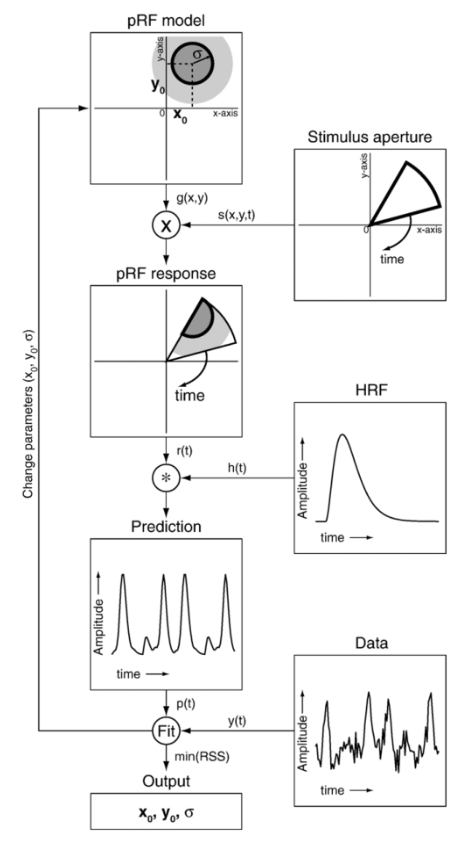
\includegraphics[scale=0.6]{../images/pRF model}
\caption{Diagrama de flujo que describe el procedimiento de estimación del modelo pRF. Tomado de [\cite{dumoulin_population_2008}]}
\label{fig:pRF}
\end{figure}

El ajuste de pRF permite derivar varias descripciones detalladas de los datos obtenidos. Entre ellas se encuentran los mapas tradicionales de excentricidad y ángulo polar, que revelan la disposición espacial y la orientación preferida de los campos receptivos en la población neuronal.


\section{Modelo lineal mixto generalizado}

Los modelos lineales mixtos generalizados (GLMM) son una poderosa clase de modelos estadísticos que combinan las características de los modelos lineales generalizados y los modelos mixtos (modelos con variables predictivas tanto fijas como aleatorias). Manejan una amplia gama de tipos de variables de respuesta y una amplia gama de escenarios en los que las observaciones se han muestreado en algún tipo de grupo en lugar de hacerlo de forma completamente independiente. Si bien no pueden hacerlo todo (un experto a veces puede elegir modelos personalizados para mayor flexibilidad (Bolker et al. 2013), los GLMM son rápidos, potentes, pueden ampliarse para manejar complejidades adicionales, como respuestas infladas a cero, y pueden suelen estar equipados con software disponible en el mercado. Las únicas desventajas reales de los GLMM se deben a su generalidad: (1) algunas recetas estándar para pruebas e inferencias de modelos no se aplican, y (2) es fácil construir modelos plausibles que son demasiado complejos para que sus datos los respalden. Los GLMM todavía son parte de la frontera estadística e incluso los expertos no conocen todas las respuestas sobre cómo usarlos, pero este capítulo intentará brindar soluciones prácticas que le permitan utilizar GLMM con sus datos.

%------------------------------------------

Modelos Lineales Mixtos Generalizados (GLMM): Son extensiones de los modelos lineales generalizados que incorporan términos aleatorios para tener en cuenta la variabilidad no explicada por las variables fijas. Se utilizan para analizar datos cuando hay correlación o agrupación en los datos, como en estudios longitudinales o con múltiples niveles de jerarquía.

